%%%%%%%%%%%%%%%%%%%%%%%%%%%%%%%%%%%%
% Slide options
%%%%%%%%%%%%%%%%%%%%%%%%%%%%%%%%%%%%

% Option 1: Slides with solutions

%\documentclass[slidestop,compress,mathserif]{beamer}
%\newcommand{\soln}[1]{#1}
%\newcommand{\solnGr}[1]{#1}

% Option 2: Handouts without solutions

\documentclass[11pt,containsverbatim,handout]{beamer}
\newcommand{\soln}[1]{ }
\newcommand{\solnGr}[1]{ }

%%%%%%%%%%%%%%%%%%%%%%%%%%%%%%%%%%%%
% Style
%%%%%%%%%%%%%%%%%%%%%%%%%%%%%%%%%%%%

\usepackage{geometry}
\usepackage{graphicx}
\usepackage{amssymb}
%\usepackage{cancel}
\usepackage{epstopdf}
\usepackage{amsmath}  	% this permits text in eqnarray among other benefits
\usepackage{url}		% produces hyperlinks
\usepackage{hyperref}	% allows for color usage in tables
\usepackage[english]{babel}
\usepackage[latin1]{inputenc}
\usepackage{colortbl}	% allows for color usage in tables
\usepackage{multirow}	% allows for rows that span multiple rows in tables
\usepackage{color}		% this package has a variety of color options
\usepackage{pgf}
\usepackage{calc}
\usepackage{ulem}
\usepackage{multicol}
\usepackage{textcomp}
\usepackage{txfonts}
\usepackage{listings}
\usepackage{tikz}
\usepackage{array}
\usepackage{wasysym}
\usepackage{fancyvrb}

%%%%%%%%%%%%%%%%
% Remove navigation symbols
%%%%%%%%%%%%%%%%

\setbeamertemplate{navigation symbols}{}

%%%%%%%%%%%%%%%%
% Get rid of fancy enumerated list bullets
%%%%%%%%%%%%%%%%

%\setbeamertemplate{enumerate items}[default]

%%%%%%%%%%%%%%%%
% Custom commands
%%%%%%%%%%%%%%%%

% two col: two columns
\newenvironment{twocol}[4]{
\begin{columns}[c]
\column{#1\textwidth}
#3
\column{#2\textwidth}
#4
\end{columns}
}

% pr: left and right parentheses
\newcommand{\pr}[1]{
\left( #1 \right)
}

% solnMult: solutions for practice questions

\newcommand{\solnMult}[1]{
\item[] \vspace{-0.59cm}
\only<1>{\item #1}
\soln{\only<2->{\item #1}}
}

% cancel
\newcommand{\cancel}[1]{%
    \tikz[baseline=(tocancel.base)]{
        \node[inner sep=0pt,outer sep=0pt] (tocancel) {#1};
        \draw[red, line width=0.5mm] (tocancel.south west) -- (tocancel.north east);
    }%
}

% removepagenumbers
%\newcommand{\removepagenumbers}{% 
%  \setbeamertemplate{footline}{}
%}



%%%%%%%%%%%%%%%%
% Graphics
%%%%%%%%%%%%%%%%

\DeclareGraphicsRule{.tif}{png}{.png}{`convert #1 `dirname #1`/`basename #1 .tif`.png}

%%%%%%%%%%%%%%%%%%%%%%%%%%%%%%%%%%%%
% Begin document
%%%%%%%%%%%%%%%%%%%%%%%%%%%%%%%%%%%%

\title[Chp 5.1: Small single sample (T distribution)]{Chp 5.1: Small single sample (T distribution)}

\begin{document}

\section{T distribution practice}
\begin{frame}
\frametitle{$t$-table practice}
\begin{itemize}
\item If $df=12$, estimate $P(T<-3.2)$.\pause
\soln{$$0.0025 ~~<~~ P(T<-3.2) ~~<~~ 0.005$$} \pause
\vfill
\item If $df=12$, determine $t$ such that $P(T>t)=0.99$.\pause
\soln{$$t = -2.68$$} \pause
\vfill
\item If $df=18$, determine $t^\star$ of a 95\% confidence interval.\pause
\soln{$$t^\star = 2.10$$} \pause
\vfill
\item If a two-tail hypothesis test has a significance level of 0.05 and a sample size $n=10$, what is the critical value $t^\star$?\pause
\soln{$$t^\star = 2.26$$}
\vfill
\end{itemize}
\end{frame}

\begin{frame}
\frametitle{$t$-table practice}
\begin{itemize}
\item If the alternative hypothesis states $\mu<100$ with a significance level $0.01$ and a sample size $n=15$, what is the critical value $t^\star$?\pause
\soln{$$t^\star = -2.62$$
An observed test statistic $t_\text{obs}$ less than $-2.62$ will cause us to reject the null.
} \pause
\vfill
\item If the alternative hypothesis states $\mu\ne 55.5$ with a significance level $0.1$ and a sample size $n=17$, what is the critical value $t^\star$?\pause
\soln{$$t^\star = 1.75$$
or, maybe, depending on how you think about it, 
$$t^\star = \pm 1.75$$ \pause
An observed test statistic $t_\text{obs}$ less than $-1.75$ or more than $1.75$ will cause us to reject the null.}
\vfill
\end{itemize}
\end{frame}


\begin{frame}
\frametitle{lower-tail $t$ test}
You will perform a single-sample \(t\) test of the alternative
hypothesis claiming \(\mu<158\). Before collecting the sample, you decide to use a significance level \(\alpha = 0.05\). The sample has the following attributes: \[\begin{aligned}
n &=& 3 \\
\bar{x} &=& 67.31 \\
s &=& 25.54
\end{aligned}\] What is your conclusion?
\end{frame}

\begin{frame} \small
We state the hypotheses: \[H_0:~~\mu = 158 \] \[H_A:~~\mu < 158 \] We
estimate the standard error (same way as with \(z\) testing).
\[SE = \frac{s}{\sqrt{n}} =  \frac{25.54}{\sqrt{3}} = 14.746\] We
calculate the \(t\) score (same way as with \(z\) testing).
\[t = \frac{67.31-158}{14.746} = -6.15 \] We determine the degrees of
freedom. \[df = n-1 = 2 \] We estimate the \(p\)-value from the \(T\)
table. \[0.01 < p\text{-value} < 0.02 \] We compare the \(p\)-value to
\(\alpha\). \[p\text{-value} < \alpha \] We make our conclusion: we
reject the null.
\end{frame}


\begin{frame}
You are given the following hypotheses: 
\begin{align*}
H_0:~~ \mu &= 140 & H_A:~~ \mu &> 140
\end{align*}
 We know that the sample standard deviation is 124 and the sample size is 10. For what sample mean would the \(p\)-value be equal to 0.001? Assume that all conditions necessary for inference are satisfied. \pause

Determine the degrees of freedom. \pause \[df = 9 \] \pause From the \(p\)-value we
find a \(t\) score from the \(t\) table. In this case, our \(p\)-value
is a one-tail probability.\pause \[t = 4.3 \] \pause We calculate the standard error. \pause
\[SE = \frac{s}{\sqrt{n}} = \frac{124}{\sqrt{10}} = 39.2 \] \pause We calculate
the sample mean that would give \(p\text{-value} = 0.001\). \pause
\[\bar{x} = \mu+t\cdot SE = 140+(4.3)(39.2) = 309 \]
\end{frame}

\begin{frame}
\frametitle{Practice}
You are given the following hypotheses: \[H_0:~~ \mu = 12\]
\[H_A:~~ \mu < 12\] We know that the sample standard deviation is 0.205
and the sample size is 20. For what sample mean would the \(p\)-value be
equal to 0.005? Assume that all conditions necessary for inference are
satisfied.
\pause
\soln{ \[df = 19 \] 

\[t = -2.86 \]

\[SE = \frac{s}{\sqrt{n}} = \frac{0.205}{\sqrt{20}} = 0.0458 \]

\[\bar{x} = \mu+t\cdot SE = 12+(-2.86)(0.0458) = 11.9 \]}

\end{frame}


\begin{frame}
A population is known to have a standard deviation \(\sigma=12\). What
is the sample size \(n\) needed to build a \(96\%\) confidence interval
with a margin of error \(ME=1\)?

\pause
{\bf Solution:}
Let's remember the formulas for confidence intervals (with known
\(\sigma\)): \[SE = \frac{\sigma}{\sqrt{n}} \]

\[CL = P(|Z| < z^{\star})\]

\[ME = z^{\star}SE \]

\[CI = \bar{x} \pm ME \]

From the confidence level \(CL=0.96\), we determine \(z^{\star}\).
\[P(|Z|<z^\star) = 0.96 \]\\
\end{frame}

\begin{frame}
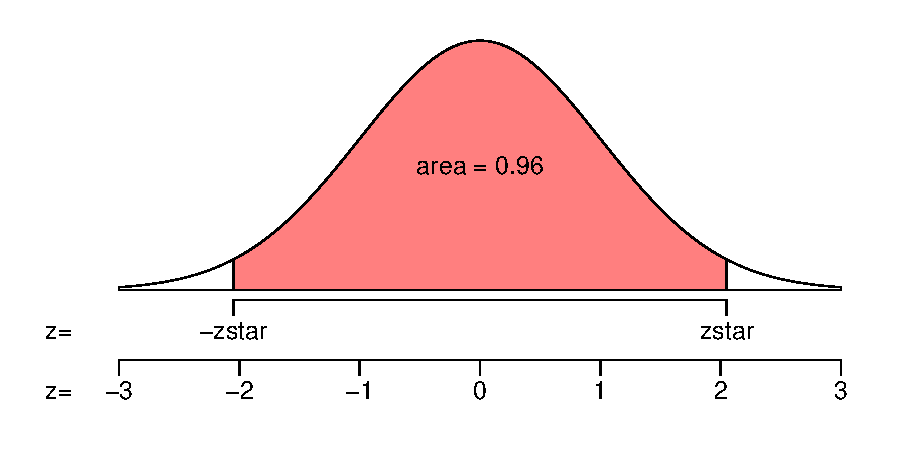
\includegraphics[scale=0.5]{CL_sketch-1a.pdf}

You can use a \(z\) table or the last row of the \(t\)-table (where
\(df=\infty\)). \[z^\star = 2.05 \] We know that \(ME=z^{\star}SE\), so
\[SE = \frac{ME}{z^{\star}} = \frac{1}{2.05} = 0.488 \]

We know that \(SE = \frac{\sigma}{\sqrt{n}}\). Let's solve for \(n\).
\[SE = \frac{\sigma}{\sqrt{n}}\] Multiply both sides by \(\sqrt{n}\).
\end{frame}

\begin{frame}
\[SE\sqrt{n}  = \sigma\] Divide both sides by \(SE\).
\[\sqrt{n} = \frac{\sigma}{SE}\] Square both sides. (Raise both sides to
the power of 2.) \[n = \left(\frac{\sigma}{SE}\right)^2\]

\[n = \left(\frac{12}{0.4878049}\right)^2 = 605.16 \] We round \(n\) up.
\[n = 606 \]
\end{frame}


\begin{frame}
A population is known to have a standard deviation \(\sigma=1.6\). What
is the sample size \(n\) needed to build a \(80\%\) confidence interval
with a margin of error \(ME=0.2\)?

\pause

\soln{
\[z^\star = 1.28 \]

\[SE = \frac{ME}{z^{\star}} = \frac{0.2}{1.28} = 0.156 \]

\[n = \left(\frac{1.6}{0.15625}\right)^2 = 104.8576 \]

\[n = 105 \]
}

\end{frame}


\begin{frame}
You will perform a single-sample \(t\) test of the alternative
hypothesis claiming \(\mu<94\). Before collecting the sample, you decide to use a significance level \(\alpha = 0.05\). The sample has the following attributes: \[\begin{aligned}
n &=& 7 \\
\bar{x} &=& 103.4 \\
s &=& 16.5
\end{aligned}\] What is your conclusion?
\vfill
\pause

\soln{The alternative is claiming $\mu<94$. This sample mean is larger than 94! This definitely does not make us tempted to reject the null. Retain the null!}
\vfill

\end{frame}


\end{document}
